% !TEX root = ../main.tex

\section{Results}
To test the perceptron compiling and training, 5 different truth tables were used, ranging from 2 to 3 inputs. The correct output was reached after 16-23 iterations of the learning algorithm. Input sizes greater than 3 was not tested, as the training time increases exponentially in time with the input size.


\begin{figure}[H]
  \begin{subfigure}[t]{.49\columnwidth}
    \begin{tabular}[b]{ccc}
      \hline
    \multicolumn{1}{l}{\textbf{Input 1}} & \multicolumn{1}{l}{\textbf{Input 2}} & \multicolumn{1}{l}{\textbf{Output}} \\
    \hline
    0                                    & 0                                    & 0                                   \\
    0                                    & 1                                    & 0                                   \\
    1                                    & 0                                    & 0                                   \\
    1                                    & 1                                    & 1 \\
    \hline
    \end{tabular}
    \caption{Truth table for the 2-input AND gate.}
    \label{and_table}
\end{subfigure}
\hfill
\begin{subfigure}[t]{.49\columnwidth}
  \centering
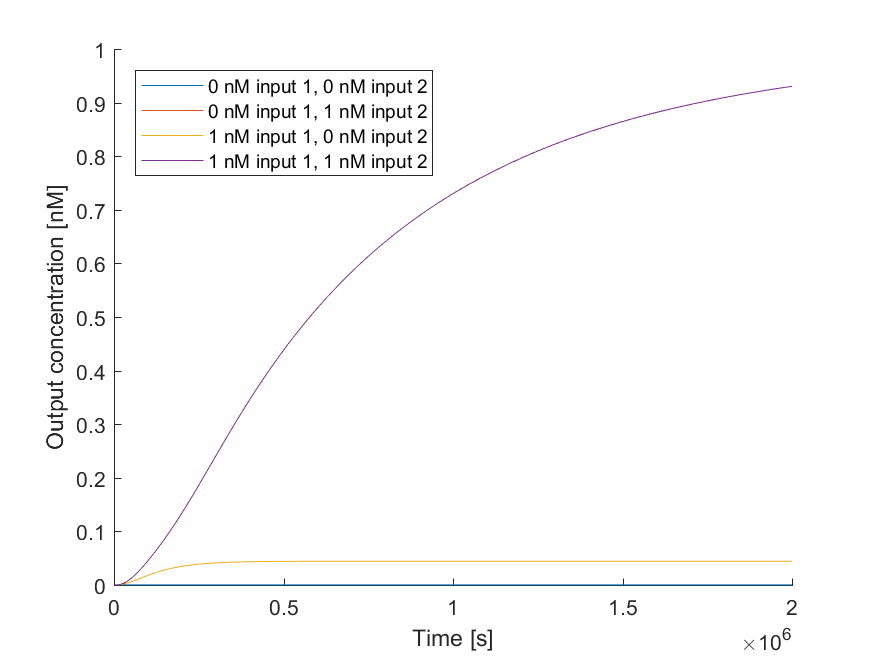
\includegraphics[width=\linewidth]{images/and_simulation.png}
\caption{.}
\label{}
\end{subfigure}
\caption{Simulation results of the trained 2-input AND gate. The network is trained to activate when both of the inputs are active. The correct output was obtained after 21 iterations of the training algorithm, with a weight of 1.9 for all inputs, and a threshold of 10.}
\end{figure}

\begin{figure}[H]
  \begin{subfigure}[t]{.49\columnwidth}
    \begin{tabular}[b]{ccc}
      \hline
    \multicolumn{1}{l}{\textbf{Input 1}} & \multicolumn{1}{l}{\textbf{Input 2}} & \multicolumn{1}{l}{\textbf{Output}} \\
    \hline
    0                                    & 0                                    & 0                                   \\
    0                                    & 1                                    & 1                                   \\
    1                                    & 0                                    & 1                                   \\
    1                                    & 1                                    & 1 \\
    \hline
    \end{tabular}
    \caption{Truth table for the 2-input OR gate.}
    \label{and_table}
\end{subfigure}
\hfill
\begin{subfigure}[t]{.49\columnwidth}
  \centering
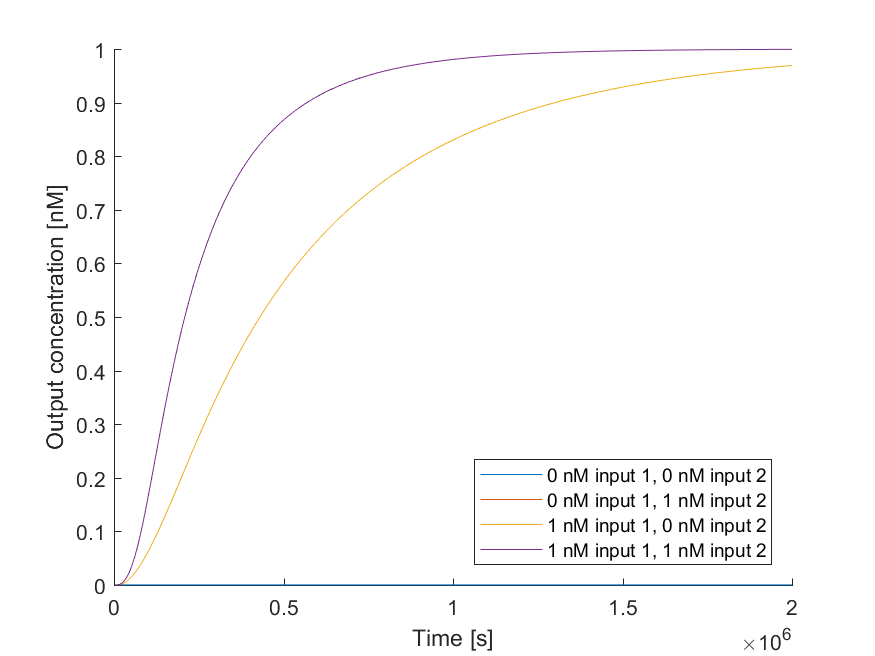
\includegraphics[width=\linewidth]{images/or_simulation.png}
\caption{.}
\label{}
\end{subfigure}
\caption{Simulation results of the trained 2-input OR gate. The network is trained to activate when one of the inputs is active. The correct output was obtained after 22 iterations of the training algorithm, with a weight of 2.1 for all inputs, and a threshold of 10.}
\end{figure}

\begin{figure}[H]
  \begin{subfigure}[t]{.49\columnwidth}
    \begin{tabular}[b]{cccc}
      \hline
    \multicolumn{1}{l}{\textbf{Input 1}} & \multicolumn{1}{l}{\textbf{Input 2}} & \multicolumn{1}{l}{\textbf{Input 3}} & \multicolumn{1}{l}{\textbf{Output}} \\
    \hline
    0 & 0                                    & 0                                    & 0                                   \\
    0 & 0                                    & 1                                    & 0                                   \\
    0 & 1                                    & 0                                    & 0                                   \\
    0 & 1                                    & 1                                    & 0                                   \\
    1 & 0                                    & 0                                    & 0                                   \\
    1 & 0                                    & 1                                    & 0                                   \\
    1 & 1                                    & 0                                    & 0                                   \\
    1 & 1                                    & 1                                    & 1                                   \\

    \hline
    \end{tabular}
    \caption{Truth table for the 3-input AND gate.}
    \label{and_table}
\end{subfigure}
\hfill
\begin{subfigure}[t]{.49\columnwidth}
  \centering
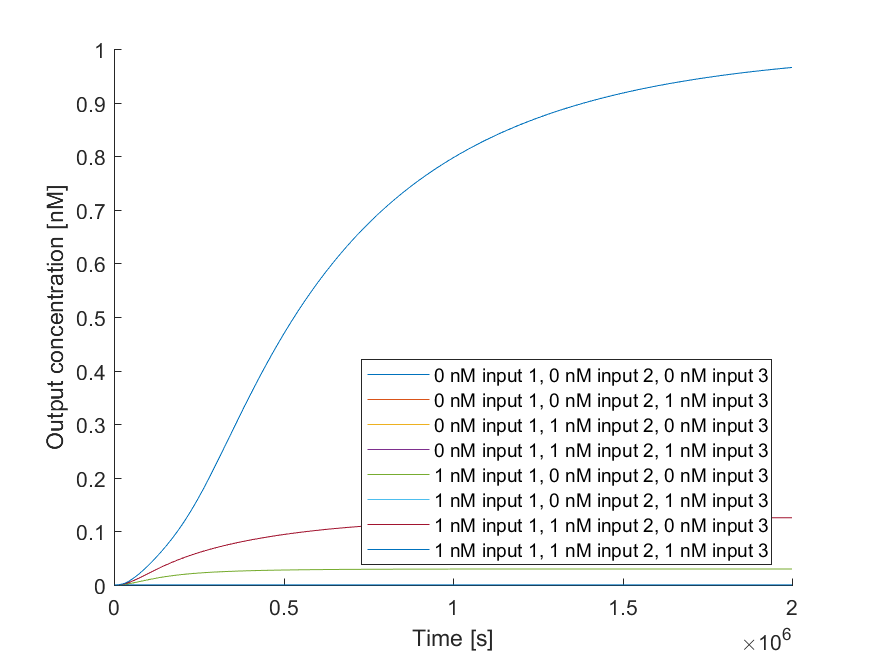
\includegraphics[width=\linewidth]{images/and_simulation_3input.png}
\caption{.}
\label{}
\end{subfigure}
\caption{Simulation results of the trained 3-input AND gate. The network is trained to activate when all of the inputs are active. The correct output was obtained after 14 iterations of the training algorithm, with a weight of 1.2 for all inputs, and a threshold of 10.}
\end{figure}

\begin{figure}[H]
  \begin{subfigure}[t]{.49\columnwidth}
    \begin{tabular}[b]{cccc}
      \hline
    \multicolumn{1}{l}{\textbf{Input 1}} & \multicolumn{1}{l}{\textbf{Input 2}} & \multicolumn{1}{l}{\textbf{Input 3}} & \multicolumn{1}{l}{\textbf{Output}} \\
    \hline
    0 & 0                                    & 0                                    & 0                                   \\
    0 & 0                                    & 1                                    & 1                                   \\
    0 & 1                                    & 0                                    & 1                                   \\
    0 & 1                                    & 1                                    & 1                                   \\
    1 & 0                                    & 0                                    & 1                                   \\
    1 & 0                                    & 1                                    & 1                                   \\
    1 & 1                                    & 0                                    & 1                                   \\
    1 & 1                                    & 1                                    & 1                                   \\

    \hline
    \end{tabular}
    \caption{Truth table for the 3-input 1-OR gate.}
    \label{and_table}
\end{subfigure}
\hfill
\begin{subfigure}[t]{.49\columnwidth}
  \centering
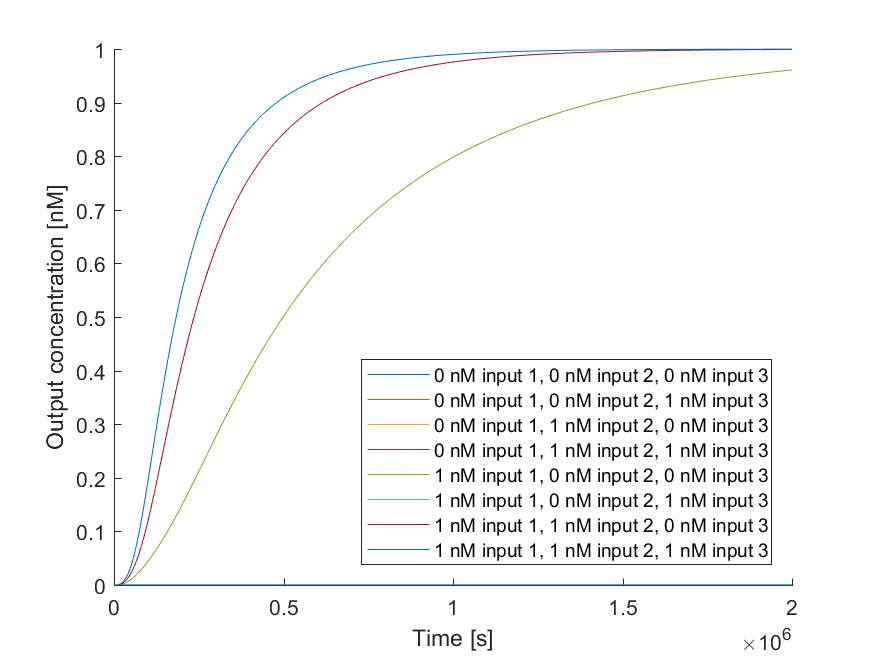
\includegraphics[width=\linewidth]{images/or_1_simulation_3input.png}
\caption{.}
\label{}
\end{subfigure}
\caption{Simulation results of the trained 3-input 1-OR gate. The network is trained to activate when at least 1 of the inputs is active. The correct output was obtained after 16 iterations of the training algorithm, with a weight of 1.3 for all inputs, and a threshold of 10.}
\end{figure}

\begin{figure}[H]
  \begin{subfigure}[t]{.49\columnwidth}
    \begin{tabular}[b]{cccc}
      \hline
    \multicolumn{1}{l}{\textbf{Input 1}} & \multicolumn{1}{l}{\textbf{Input 2}} & \multicolumn{1}{l}{\textbf{Input 3}} & \multicolumn{1}{l}{\textbf{Output}} \\
    \hline
    0 & 0                                    & 0                                    & 0                                   \\
    0 & 0                                    & 1                                    & 0                                   \\
    0 & 1                                    & 0                                    & 0                                   \\
    0 & 1                                    & 1                                    & 1                                   \\
    1 & 0                                    & 0                                    & 0                                   \\
    1 & 0                                    & 1                                    & 1                                   \\
    1 & 1                                    & 0                                    & 1                                   \\
    1 & 1                                    & 1                                    & 1                                   \\

    \hline
    \end{tabular}
    \caption{Truth table for the 3-input 2-OR gate.}
    \label{and_table}
\end{subfigure}
\hfill
\begin{subfigure}[t]{.49\columnwidth}
  \centering
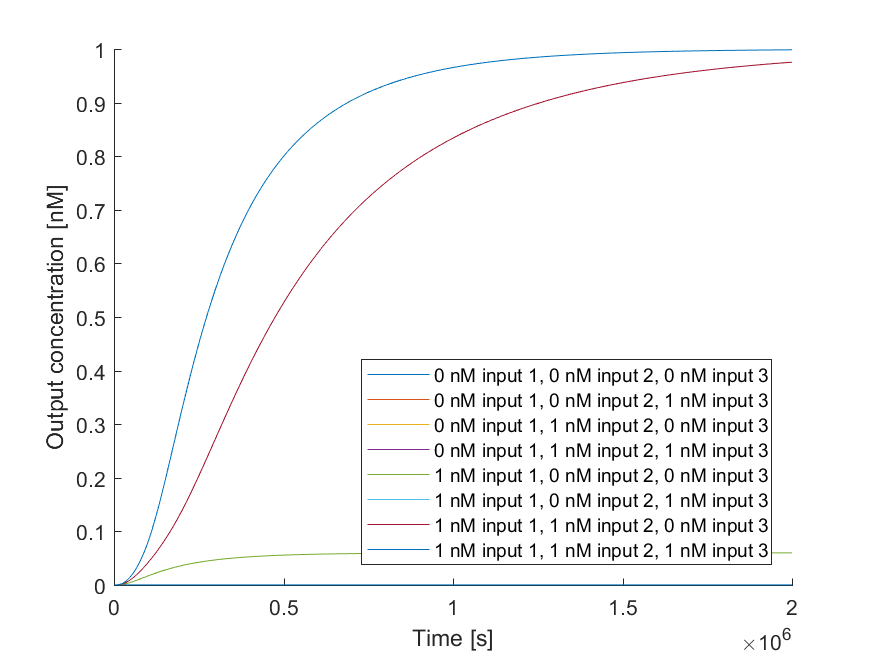
\includegraphics[width=\linewidth]{images/or_2_simulation_3input.png}
\caption{.}
\label{}
\end{subfigure}
\caption{Simulation results of the trained 3-input 2-OR gate. The network is trained to activate when at least 2 of the inputs is active. The correct output was obtained after 15 iterations of the training algorithm, with a weight of 1.3 for all inputs, and a threshold of 10.}
\end{figure}
